%% LaTeX Beamer presentation template (requires beamer package)
%% see http://bitbucket.org/rivanvx/beamer/wiki/Home
%% idea contributed by H. Turgut Uyar
%% template based on a template by Till Tantau
%% this template is still evolving - it might differ in future releases!

\documentclass{beamer}

\mode<presentation>
{
\usetheme{Warsaw}

\setbeamercovered{transparent}
}

\usepackage[russian]{babel}
\usepackage[utf8]{inputenc}

% font definitions, try \usepackage{ae} instead of the following
% three lines if you don't like this look
\usepackage{mathptmx}
\usepackage[scaled=.90]{helvet}
\usepackage{courier}


\usepackage[T1]{fontenc}


\title{Построение автоконфигурируемой сети мехатронных устройств для задач
территориально-распределённого управления}

%\subtitle{}

% - Use the \inst{?} command only if the authors have different
%   affiliation.
%\author{F.~Author\inst{1} \and S.~Another\inst{2}}
\author{В.П. Андреев\inst{1}, К.Б. Кирсанов\inst{2}, П.Ф.Плетенев\inst{1} }
% - Use the \inst command only if there are several affiliations.
% - Keep it simple, no one is interested in your street address.
\institute[Universities of]
{
\inst{1}
МГТУ ''Станкин''
\and
\inst{2}
ИПМ им. Келдыша, РАН

}
\date{09.10.2015 / ЭР-2015}


% This is only inserted into the PDF information catalog. Can be left
% out.
%\subject{Talks}



% If you have a file called "university-logo-filename.xxx", where xxx
% is a graphic format that can be processed by latex or pdflatex,
% resp., then you can add a logo as follows:

% \pgfdeclareimage[height=0.5cm]{university-logo}{university-logo-filename}
% \logo{\pgfuseimage{university-logo}}



% Delete this, if you do not want the table of contents to pop up at
% the beginning of each subsection:
%\AtBeginSubsection[]
%{
%\begin{frame}<beamer>
%\frametitle{Outline}
%\tableofcontents[currentsection,currentsubsection]
%\end{frame}
%}

% If you wish to uncover everything in a step-wise fashion, uncomment
% the following command:

%\beamerdefaultoverlayspecification{<+->}
  
\begin{document}

\begin{frame}
\titlepage
\end{frame}

\begin{frame}
\frametitle{Оглавление}
\tableofcontents
% You might wish to add the option [pausesections]
\end{frame}


\section{Введение}
\subsection{Связующее ПО в задачах мобильной робототехники}
\begin{frame}
\frametitle{Что такое связующее ПО (middleware)}
Связующее ПО это фреймворки и SDK, реализующие
утилиты и базовые функции для разработки и тестирования программных модулей и
различных мехатронных компонент. Они задают спецификацию для ''выражения''
модели управления мобильным роботом в компьютерных терминах и включают описания
моделей для:

\vskip0pt plus.5fill

\begin{itemize}
  \item Роботов и мехатронных компонент
  \item Cхемы именования и адресации
  \item Способов взаимодействия
\end{itemize}

\end{frame}


\begin{frame}
\frametitle{Что такое связующее ПО (middleware)}
\framesubtitle{Примеры}
\begin{itemize}
\item<1> \textbf{ROS Robotic Operating System}
\item<1> \textbf{Microsoft Robotics Studio} 
\item<1> \textbf{Player Project} 
\item<1> \textbf{ORCA2} 
\item<1> \textbf{LAAS/GenoM} 
\item<1> \textbf{Marie} 
\item<1> \textbf{URBI} 
\item<1> \textbf{Webots} 
\item<1> \textbf{RoboJRE}
\item<1> \textbf{OROCOS}
\item<1> \textbf{Проприетарные SDK для конкретных роботов Festo
ABB, Kuka и т.д.}
\end{itemize}
\end{frame}

\subsection{Модель робота в ПО}
\begin{frame}
\frametitle{Роботы и мехатронные компоненты в терминах ПО}

\begin{itemize}
\item Роботы и мехатронные компоненты абстрагируются в терминах конечных
автоматов
\item В результате процедура управления трансформируется в
изменение состояний конечных автоматов
\item Изменения состояний реализуются с помощью механизма сообщений, синхронных
или асинхронных
\end{itemize}


\center{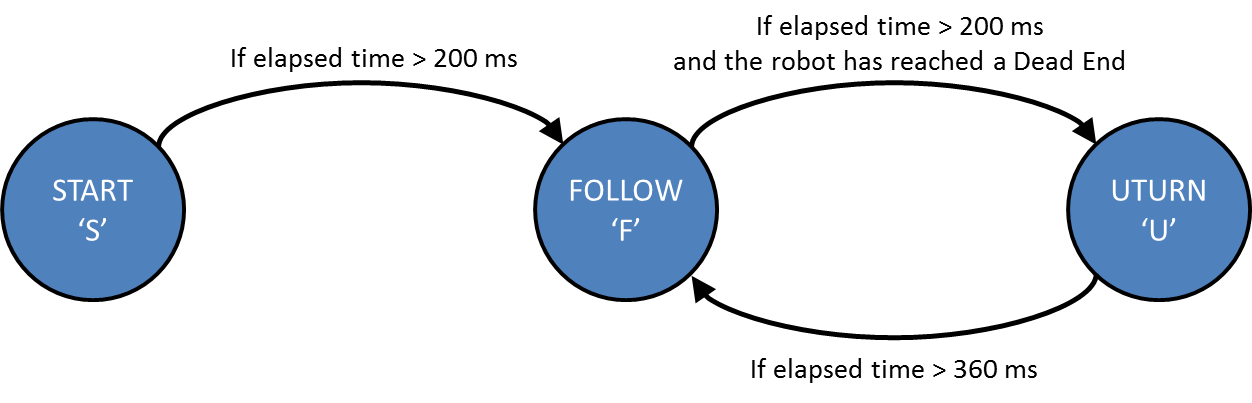
\includegraphics[width=7cm]{simplefsmdiagram.png}}

\end{frame}

\begin{frame}
\frametitle{Необходимые процедуры}

\begin{itemize}
\item Именование и адресация - как обратиться из программы к конкретному
устройству
\item Механизм сообщений - как прочитать или изменить состояние конечного
автомата
\item Агрегирование и комплексирование - как собрать (в рамках ПО) робота
или группу роботов из множества устройств
\end{itemize}


Ближайший аналог - WWW и интернет: \textbf{именование и адресация} это DNS
серверы и адреса, \textbf{механизм сообщений} это
HTTP протокол, \textbf{ агрегирование и комплексирование} это браузер, который
с помощью серии HTTP запросов формирует и показывает веб-страницу
\end{frame}
\section{Предлагаемая архитектура}

\begin{frame}
\frametitle{Предлагаемая архитектура}

\framesubtitle{Ограничения}

\begin{itemize}
  \item Мультиплатформенность - x86, arm, avr и независимость от языка
  программирования (ЯП)
  \item Восстановление после сбоев и автоконфигурируемость
  \item Малый размер кодовой базы, чтобы уместиться в памяти бортовой ЭВМ
  \item Быстрое прототипирование
\end{itemize}

\center{
	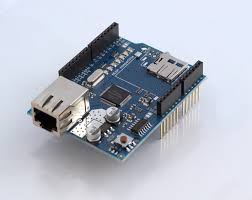
\includegraphics[width=3cm]{arduino.jpg}
	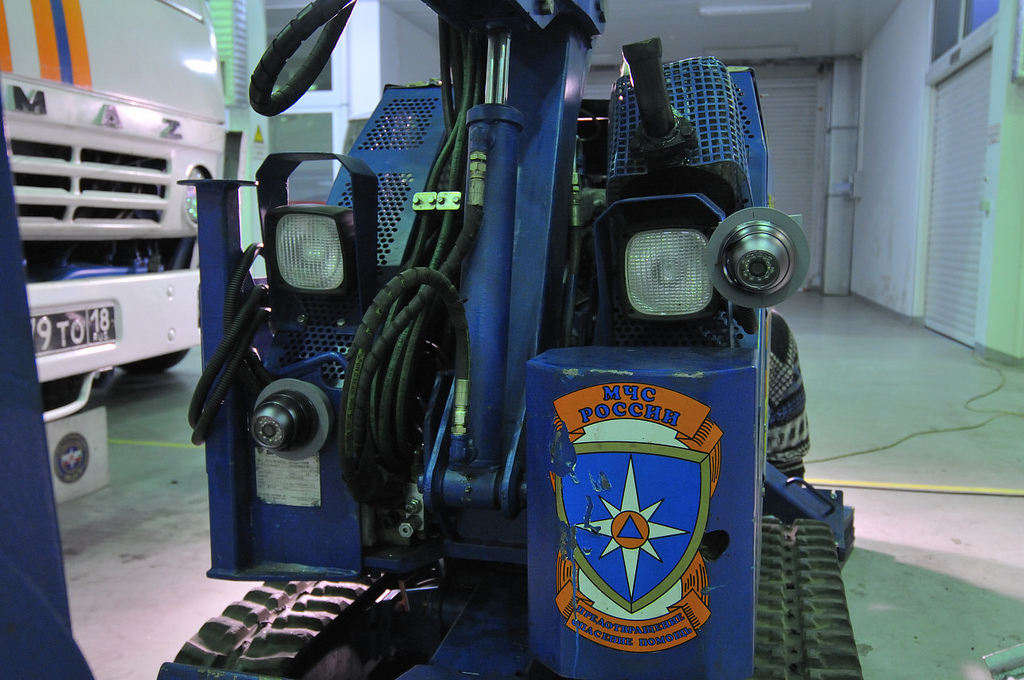
\includegraphics[width=3.5cm]{brokk.jpg}
	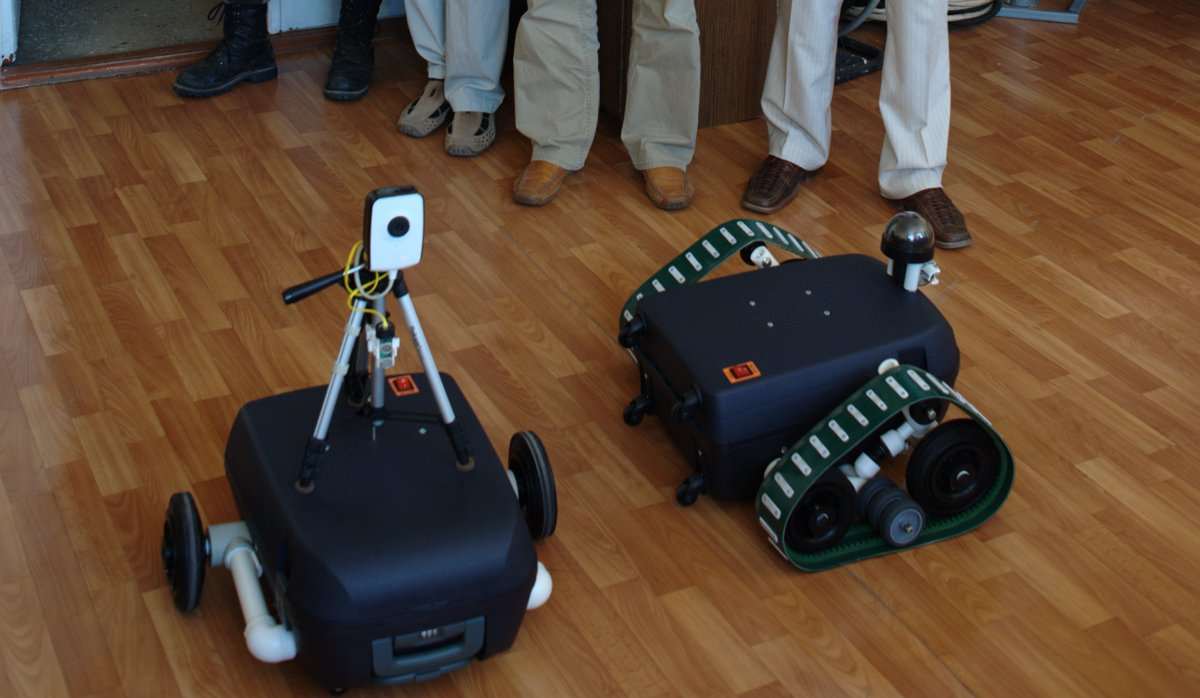
\includegraphics[width=4cm]{amur2.jpg}
		
}
\small{
Сбои вызваны кратковременным покиданием области радио-видимости,
переподключением оборудования или переходом в другую беспроводную сеть.
}
\end{frame}

\subsection{Именование и адресация}
\begin{frame}
\frametitle{Схема именования и адресации}
Используется иерархическая структура с уникальными идентификаторами:
\begin{itemize}
  \item Может быть построено отображение в строку:
  \emph{'Place->Laboratory->Robot->Device->SubDevice'} или
  \emph{'ip addres>Port'}
  \item Удобство реализации рекурсивных алгоритмов
\end{itemize}
\center{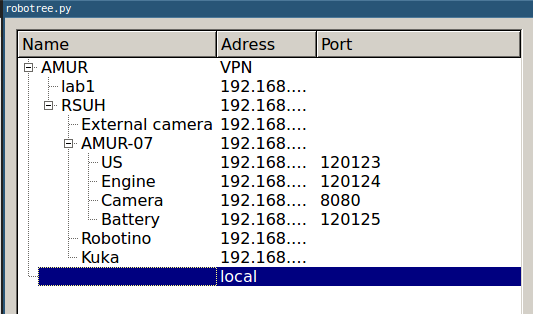
\includegraphics[width=5cm]{tree.png}}

\end{frame}

\subsection{Поиск}
\begin{frame}
\frametitle{Процедура поиска}
\begin{itemize}
\item Прежде чем начать работать с чем-либо нужно это ``найти``. 
В реальном мире эта процедура очевидна, но в рамках ПО ее необходимо явным
образом описать.
\item Для этого реализована специализированная подсистема - Сервер Имен (СИ),
сопоставляющая имена мехатронных компонент и способы доступа к ним.
\item Каждое устройство автоматически регистрируется при запуске в своем
эксземпляре СИ.
\item Каждый СИ периодически сканирует известные ему локальные сети в
поисках новых устройств или перезарегистрировавшихся старых.
\end{itemize}
\end{frame}

\begin{frame}
\framesubtitle{Реализация процедур регистрации, поиска и взаимодействия}
\center{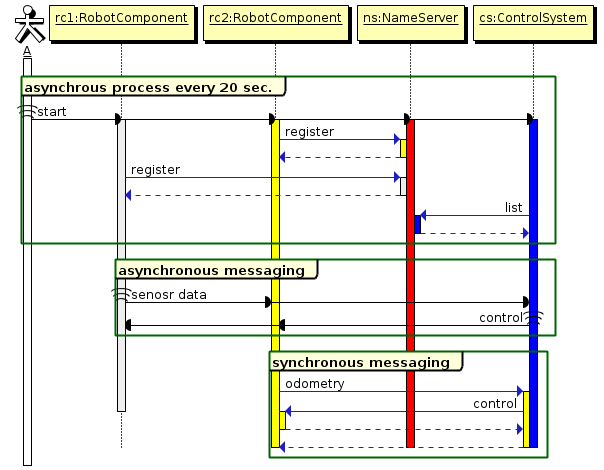
\includegraphics[width=8cm]{nameserver.png}}
\end{frame}

\subsection{Система сообщений}
\begin{frame}
\frametitle{Традиционный подход}
\begin{itemize}
	\item<1>Основные языки разработки: C, Java, C\# .
	\item<1>Мультиагентная архитектура - каждый мехатронный компонент
	представляется отдельным агентом, а робот - их композицией.
	\item<1>Агенты взаимодействуют через удаленный вызов процедур (RPC - Remote
	Proceduree call) или простейшие протоколы.
\end{itemize}
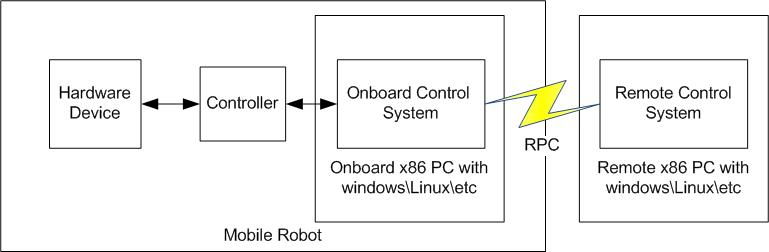
\includegraphics[width=10.5cm]{rpc0.jpg}
\end{frame}


\begin{frame}
\frametitle{Недостатки традиционного подхода}
\begin{itemize}
\item<1>Осуществление вызовов RPC требует существования соответствующих функций
со стороны бортовой ЭВМ. При этом в процессе разработки они часто модифицируются
или добавляются.
\item<1>ПО на бортовой ЭВМ реализуется на компилируемых языках.
\end{itemize}
 
\begin{itemize}
\item<1>Трудно разрабатывать - создание и тестирование алгоритмов требует
длительной процедуры перезапуска.
\item<1>Трудно отлаживать - невозможно обновлять программный код во время работы
системы.
\end{itemize}
\end{frame}

\begin{frame}
\frametitle{Предлагаемый подход}

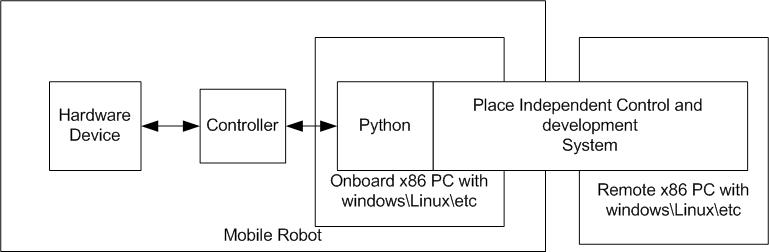
\includegraphics[width=10.5cm]{rpc1.jpg}
\begin{itemize}
 \item<1>В бортовую ЭВМ вводится промежуточный слой динамического
 интерпретируемого языка программирования (в нашей реализации - python), который
 используется для компенсации вышеназванных недостатков
\end{itemize}
\end{frame}

\begin{frame}
\begin{itemize}
  \item На нижнем уровне используется библиотека 0MQ 
  \item На верхнем уровне идет обмен сообщениями, сериализованными в ASCII
  формат JSON
  \item Каждое сообщение содержит метку локального и логического времени
  (становится актуальным при использовании mesh-сетей).
\end{itemize}
\center{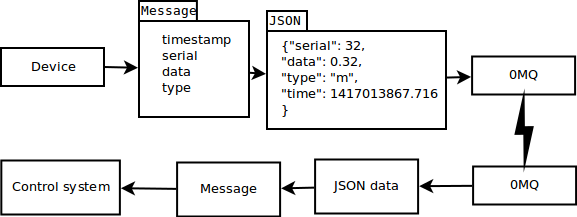
\includegraphics[width=8cm]{messaging.png}}
\end{frame}

\subsection{Шлейф измерений}
\begin{frame} 
\frametitle{Шлейф измерений}
\begin{itemize}
  \item Когда устройство отключается от сети - не происходит обрыва на верхнем
  уровне (т.е. уровне ПО, работающем с системой сообщений).
  \item Когда устройство возвращается в сеть - нет
  необходимости в отдельной процедуре восстановления.
  \item Все передаваемые сообщения хранятся в миниатюрных локальных БД
  (являются составной частью Сервера Имен), благодаря чему появляется
  возможность запросить старые данные или данные, недоступные во время сетевого сбоя.
\end{itemize}
\end{frame}

\begin{frame} 
\frametitle{Шлейф измерений}
\center{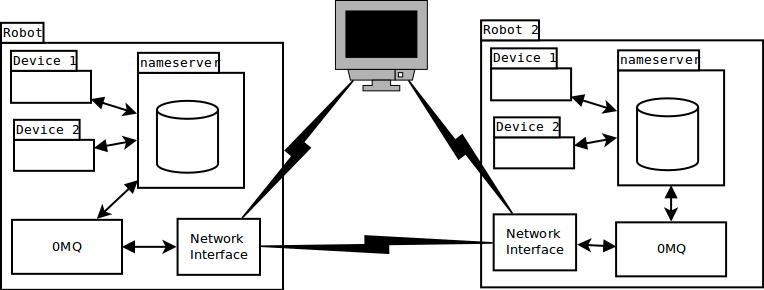
\includegraphics[width=11cm]{messaging2.png}}

\end{frame}


\section{Заключение}
\begin{frame}

\frametitle{Заключение}

\framesubtitle{Частота обмена сообщениями в сети WiFi между пультом управления и
бортовой ЭВМ}
\center{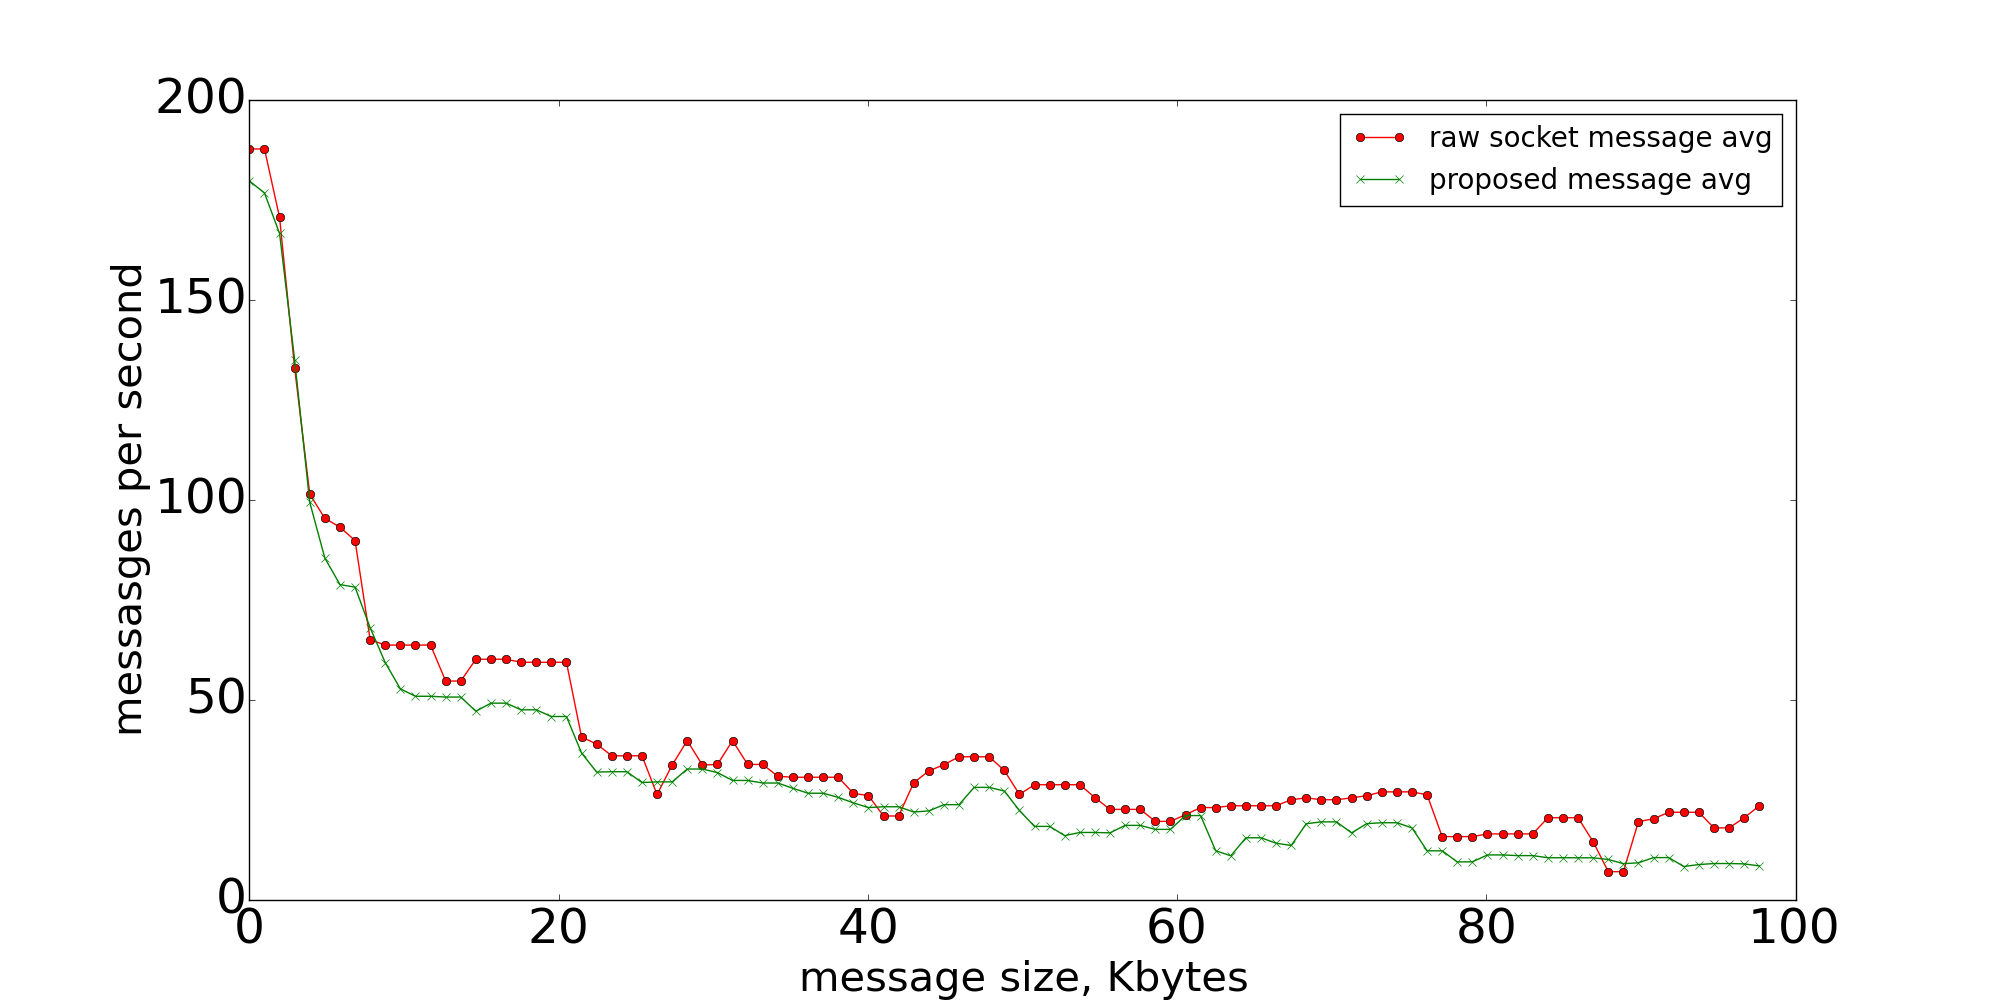
\includegraphics[width=11cm]{ping3.png}} \\
100 последовательных случайных синхронных сообщений (всего 200) на каждой
итерации.
\end{frame}

\begin{frame}
\frametitle{Заключение}
\begin{itemize}
  \item Предложена новая архитектура ПО, позволяющая ускорить
  процесс разработки и отладки. Ускорение достигается за счет использования
  промежуточного слоя из интерпретируемого динамического языка и реализованной
  схемы обмена сообщениями.
  \item Low performance of interpreted languages is not the bottleneck
   because core resources are spent on tasks of other
   subsystems.
\end{itemize}
\end{frame}



\end{document}